% !Mode:: "TeX:UTF-8"
% !TEX program  = xelatex

\section{FaPN Based APP}
%完整的应用在移动端的语义分割APP应该包括了客户端和服务器端,移动端主要负责为用户提供易于交互的UI界面,获取图像和进行相关信息的设置;服务器端主要负责对数据的存储和模型的训练和模型的执行。其中在本paper中模型的训练服务器不同于模型执行服务器。客户端和服务器端双端模式有几个优点,包括:1)提升了功能的可维护性和易用性,通过前后端解耦,用户无需关心服务的底层逻辑,且APP形式更加易于操作,便于服务的扩展和普及。2)APP和服务器端收发的过程中实现了MD5加密,从而保证了数据在传输过程中的安全性。3)合理分配了信息与任务,客户端为用户提供了可供选择的选项,而服务器端只需处理和收发信息。
The semantic segmentation APP of a complete application on the mobile terminal should include client and server. 
The mobile terminal is mainly responsible for providing users with an easy-to-interact UI interface, obtaining images, and setting related information. 
The server-side is mainly responsible for data storage and models. Training and model execution. The training server of the model in this paper is different from the model execution server. The client-side and server-side double-end mode has several advantages, including: 

1). Improves the maintainability and ease of use of functions. Through the decoupling of the front and back ends, the user does not need to care about the underlying logic of the service, and the APP form is easier to operate, Facilitate the expansion and popularization of services. 

2). MD5 encryption is implemented in the process of sending and receiving between the APP and the server, thereby ensuring the security of data during transmission. 

3). Information and tasks are reasonably allocated, the client-side provides users with options to choose from, while the server-side only needs to process and send and receive information.

\subsection{Server End Construction}

\subsubsection{Model Training}

%此部分主要介绍了在不同的数据集上使用不同的backbone网络+FaPN进行训练,并评估了在数据集的测试集上的性能。

In this section, I mainly introduce the training process of different backbone networks with FaPN on different datasets and evaluates the performance on the test set of the dataset.

\textbf{COCO 2017 Dataset: }MS COCO \cite{lin2014microsoft} consists of over 100K images with different objects and annotations including bounding boxes and segmentation masks. I use the train2017 set (about 118K images) for training and report the results val2017 set (5K images) for comparison. For both object detection and instance segmentation tasks, there are 80 categories; for panoptic segmentation tasks, there are 80 stuff and 53 stuff classes annotated.

%TT100K数据集是腾讯和清华一起合作制作的交通标志数据集,其包含约10K的各类国内交通标识的图像。经过计算,训练数据集总共包含16527个实例,测试数据集包含8190个实例。TT100K是国内相对较完整,覆盖种类完善的交通标识数据集之一,其应用场景是目标检测,数据集标注只包括图像对应的位置,因此只能用于目标检测的相关训练。图片的标注文件格式是json,原数据集存在类别不均衡的问题,一些多存在于山区,险路的交通标识相对更少。原数据集格式不符合Detectron2训练要求,需要将其转换为Detectron2要求的COCO格式。具体方式是先读取原数据集的json标注文件,原文件包含了图像对应的类别和位置信息,然后将读取到的相关信息转换为COCO格式即可。
\textbf{TT100K dataset in COCO format:} The TT100K dataset is a traffic sign dataset jointly produced by Tencent and Tsinghua, which contains about 10K images of various domestic traffic signs. After calculation, the training dataset contains a total of 16527 instances, and the test dataset contains 8190 instances. TT100K is one of the relatively complete and comprehensive traffic sign datasets in China. Its application scenario is target detection. The annotation of the dataset only includes the position corresponding to the image, so it can only be used for training related to target detection. The annotation file format of the pictures is JSON. The original data set has the problem of unbalanced categories. Some of them are mostly in mountainous areas, and there are relatively few traffic signs on dangerous roads. The format of the original dataset does not meet the training requirements of Detectron2, and it needs to be converted to the COCO format required by Detectron2. The specific method is to first read the JSON annotation file of the original dataset, which contains the category and location information corresponding to the image, and then convert the read-related information into COCO format.

\begin{table}[htb]
	% h-here,t-top,b-bottom,优先级依次下降
		\begin{center}
		% 居中
			\caption{Notations}\label{Notation}
			\begin{tabular}{|c|l|} % 三线表不能有竖线,l-left,c-center,r-right
				\toprule
				\textbf{Notation} & \textbf{Definition}\\
				\hline
				$f_a(·)$ & feature aligned procedure\\
				$f_s(·)$ & feature selection procedure\\
				$f_m(·)$ & feature importance modeling procedure\\
				$P^u_i$ & unaligned feature i in upsampled layer\\
				$\textbf{z}$ & importance value set\\
				$\Delta_i$ & offset distance\\
				$C_i$ & unaligned feature i\\
				$H$ & height of the feature map\\
				$W$ & width of the feature map\\
				$x_\textbf{p}$ & feature in the given position p\\
				$\Delta\textbf{p}_n$&tuple of the additional offset\\
				$f_i$&aligned feature i\\
				$AP$&average precision\\
				\bottomrule
			\end{tabular}
		\end{center}
	\end{table}

The deformable convolution is used in the feature aligned procedure. It can be mathematically presented as Equation(\ref{con:deformableConvolution}).



\begin{equation}
    \begin{aligned}
    \hat{x}_\textbf{p}= \sum_{n = 1}^{N}w_n * x_{\textbf{p}+\textbf{p}_n},
    \label{con:deformableConvolution}
    \end{aligned}
\end{equation}

input $\textbf{c}_i \in \mathbb{R}^{H_i * W_i}$ is the feature map and the conv layer with $k * k$. The output $\hat{x}_\textbf{p}$ is the feature in the given position $\textbf{p}$. Then it can be calculated according to the sum of the convolution procedure. However, for the FAM module, the additional offset distance is added, so the Equation(4) can be reformulated as Equation(\ref{con:famConvolution}).

\begin{equation}
    \begin{aligned}
    \hat{x}_\textbf{p}= \sum_{n = 1}^{N}w_n * x_{\textbf{p}+\textbf{p}_n+\Delta\textbf{p}_n},
    \label{con:famConvolution}
    \end{aligned}
\end{equation}

where the $\Delta\textbf{p}_n$ is a tuple $[h, w] \in [(-H_i, H_i), (-W_i, W_i)]$.

\begin{algorithm}[htbp]
	\caption{Pseudo-Code of Feature Aligned Module} 
	\label{alg1} 
	\begin{algorithmic}
		\REQUIRE 
        The input channel, $C_{in}$;
		\ The output channel, $C_{out}$;
		\ The bottom-up feature map, $f_m$;
		\ The top-down feature map, $f_t$;
		\ENSURE 
        The aligned feature, $\hat{f}_i$;
		\STATE Execute the FSM module with $C_{in}$ and $C_{out}$.
		\STATE Initialize the offset layer with nn.Conv2d.
		\STATE Use nn.Relu as the activation function.
		\IF{$f_m$'s size not equals to the size of $f_t$}
        \STATE Use F.interpolate to upsample the $f_t$.
		\ENDIF 
		\STATE Select important features $\hat{f}_t$ through FSM module.
		\STATE $\hat{f}_i \gets \hat{f}_t + f_m$.

	\end{algorithmic} 
\end{algorithm}

\begin{algorithm}[htbp]
	\caption{Pseudo-Code of Feature Selection Module} 
	\label{alg2} 
	\begin{algorithmic}
		\REQUIRE 
        The input channel, $C_{in}$;
		\ The output channel, $C_{out}$;
		\ENSURE The selected feature, $\hat{f}_i$;
		\STATE Use F.avg\_pool2d to get the result of average pool of input feature map.
		\STATE Use nn.Conv2d to get the feature vector $\textbf{z} =  [z_1, z_2, ..., z_D]$.
		\STATE Multiply the $\textbf{z}$ with input feature map, get the result $x$.
		\STATE $C_{out} \gets nn.Conv2d(C_{in}, C_{out}, 1, x)$. 

	\end{algorithmic} 
\end{algorithm}

%FaPN在FPN的基础上添加了feature selection module和feature aligned module,在此基础上可以使用包括Faster R-CNN,PointRend,Mask R-CNN等多种backbone网络,并在Object Detection,Cityscapes Semantic Segmentation,COCO Instance Segmentation上都相对FPN取得了1.2%-2.6%的提升 [5]。本文基于FaPN的模块在上述backbone网络中都针对COCO2017数据集进行了训练。训练参数如下:(训练参数)

FaPN adds feature selection module \cite{hu2018squeeze} and feature aligned module based on FPN. Compared with FPN, Instance Segmentation has achieved 1.2\%-2.6\% improvement \cite{huang2021fapn}. The FaPN-based modules in this paper are all trained on the COCO2017 dataset in the aforementioned backbone networks. The training parameters are presented in the relevant environment for the training and running section.

%针对上述几种模型的性能评估,Average Precision,也即AP值是主要评价指标,AP值可以按照检测目标的大小分为APs,APm,APl;APs,APm,APl分别表示对于small, medium and large objects的检测效果。mIoU,也就是mean Intersection-over-Union,主要用于评估语义分割的性能。

For the performance evaluation of the above-mentioned models, Average Precision, that is, the AP value is the main evaluation index. The AP value can be divided into $AP_s$, $AP_m$, and $AP_l$ according to the size of the detection target; $AP_s$, $AP_m$, and $AP_l$ respectively represent small, medium and large The detection effect of objects. mIoU, also known as mean Intersection-over-Union, is mainly used to evaluate the performance of semantic segmentation \cite{padilla2021comparative}.

%miou,两框交集/两框并集
$$ mIoU = \frac{1}{k+1} \sum_{i=0}^{k}\frac{p_{ii}}{\sum_{i=0}^{k}p_{ij}+\sum_{j=0}^{k}p_{ji}-p_{ii}}$$

$$AP = \frac{1}{N}\sum_{n=1}^{N}Pr_{interp}(R_r(n))\ $$
$$AP_s = AP (small\ objects\ that\ area < 32^2)$$
$$AP_m = AP (medium\ objects\ that\ 32^2 < area < 96^2)$$
$$AP_l = AP (large\ objects\ that\ area > 96^2)$$

\begin{figure}[htb]
    \centering
    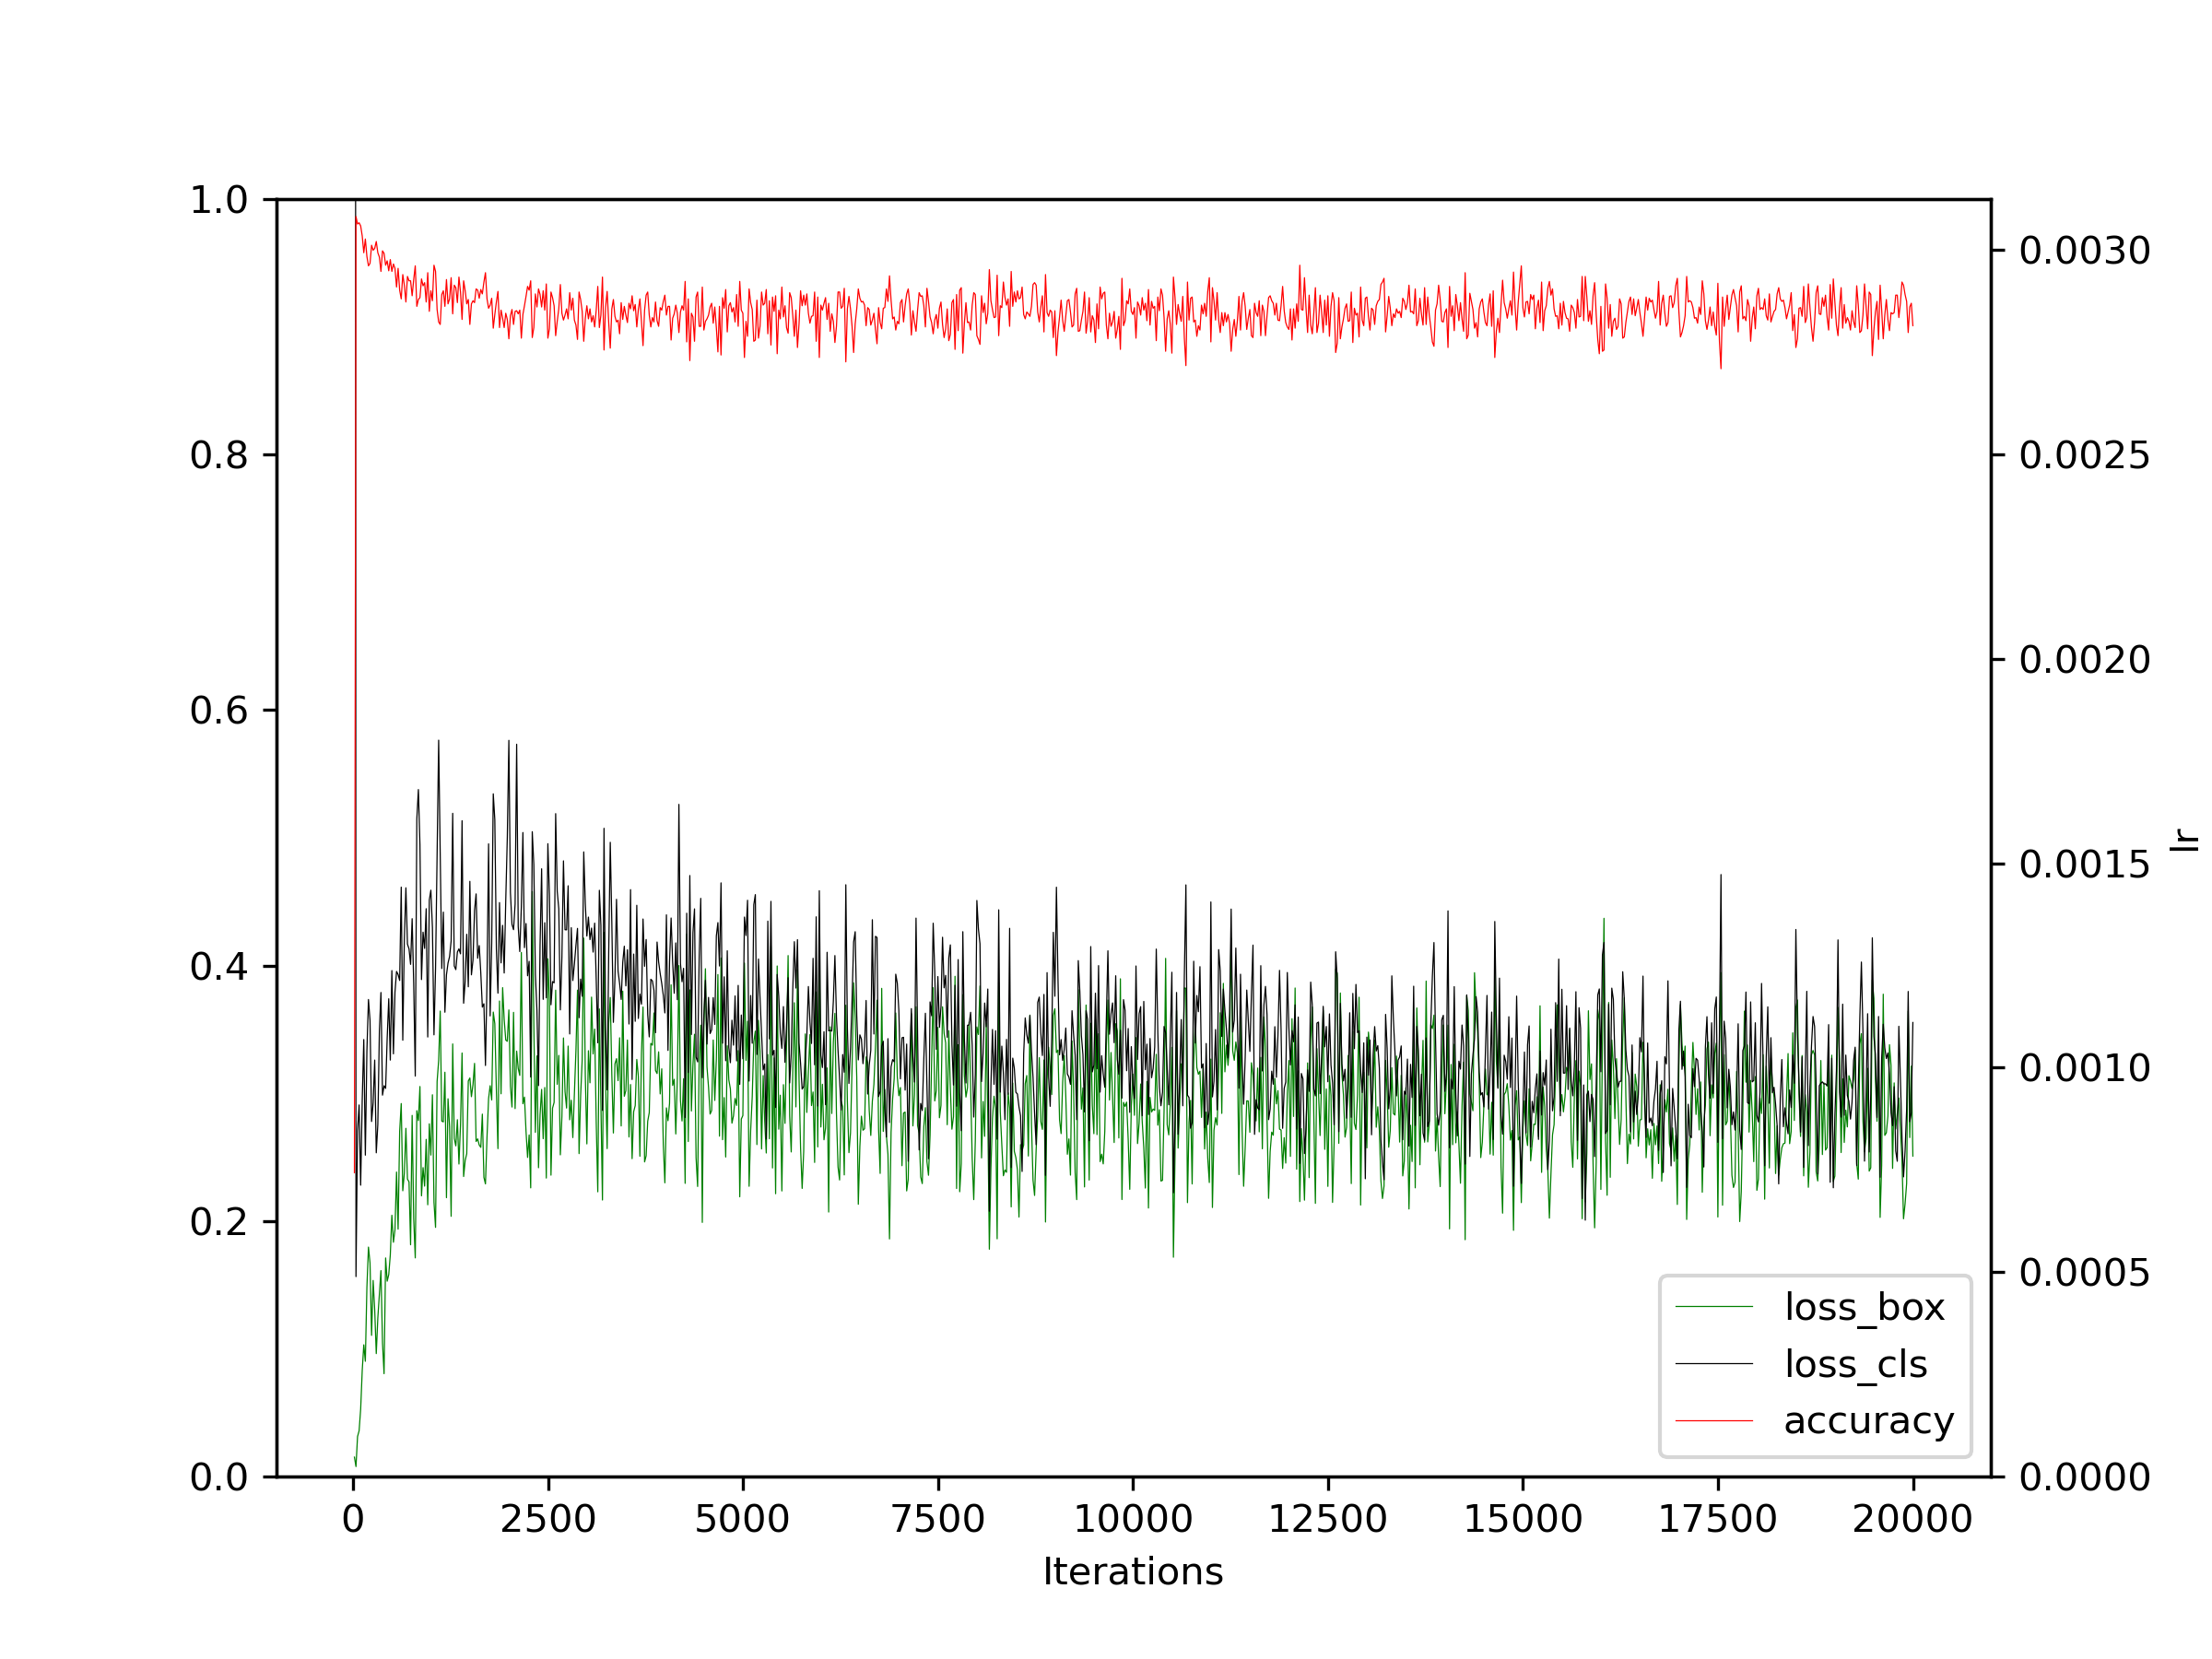
\includegraphics[width=1\textwidth]{figures/mask_rcnn_r_50_fapn_1x_20000iter.png}
    \caption{Mask RCNN \& FaPN with 20000 interactions}\label{mask_rcnn_r_50_fapn_1x_20000iter}
\end{figure}

%可以看到,在进行20000iteration,默认参数的训练后,准确率稳定在了95\%的水平,而loss_box 和 loss_cls都熟练到了0.002以内,具有较好的性能。

It can be seen that after 20000 iterations and default parameter training, the accuracy rate has stabilized at the level of 95\%, and both loss box and loss cls are proficient to within 0.002, with sufficient performance for use.


%随后对Faster RCNN在加入FaPN模块后,在10000 iterations上进行了训练,得到了下图所示的结果:

Then Faster RCNN \cite{ren2015faster} was trained on 10,000 iterations after adding the FaPN module, and the results shown in the figure below were obtained.

\begin{figure}[htb]
    \centering
    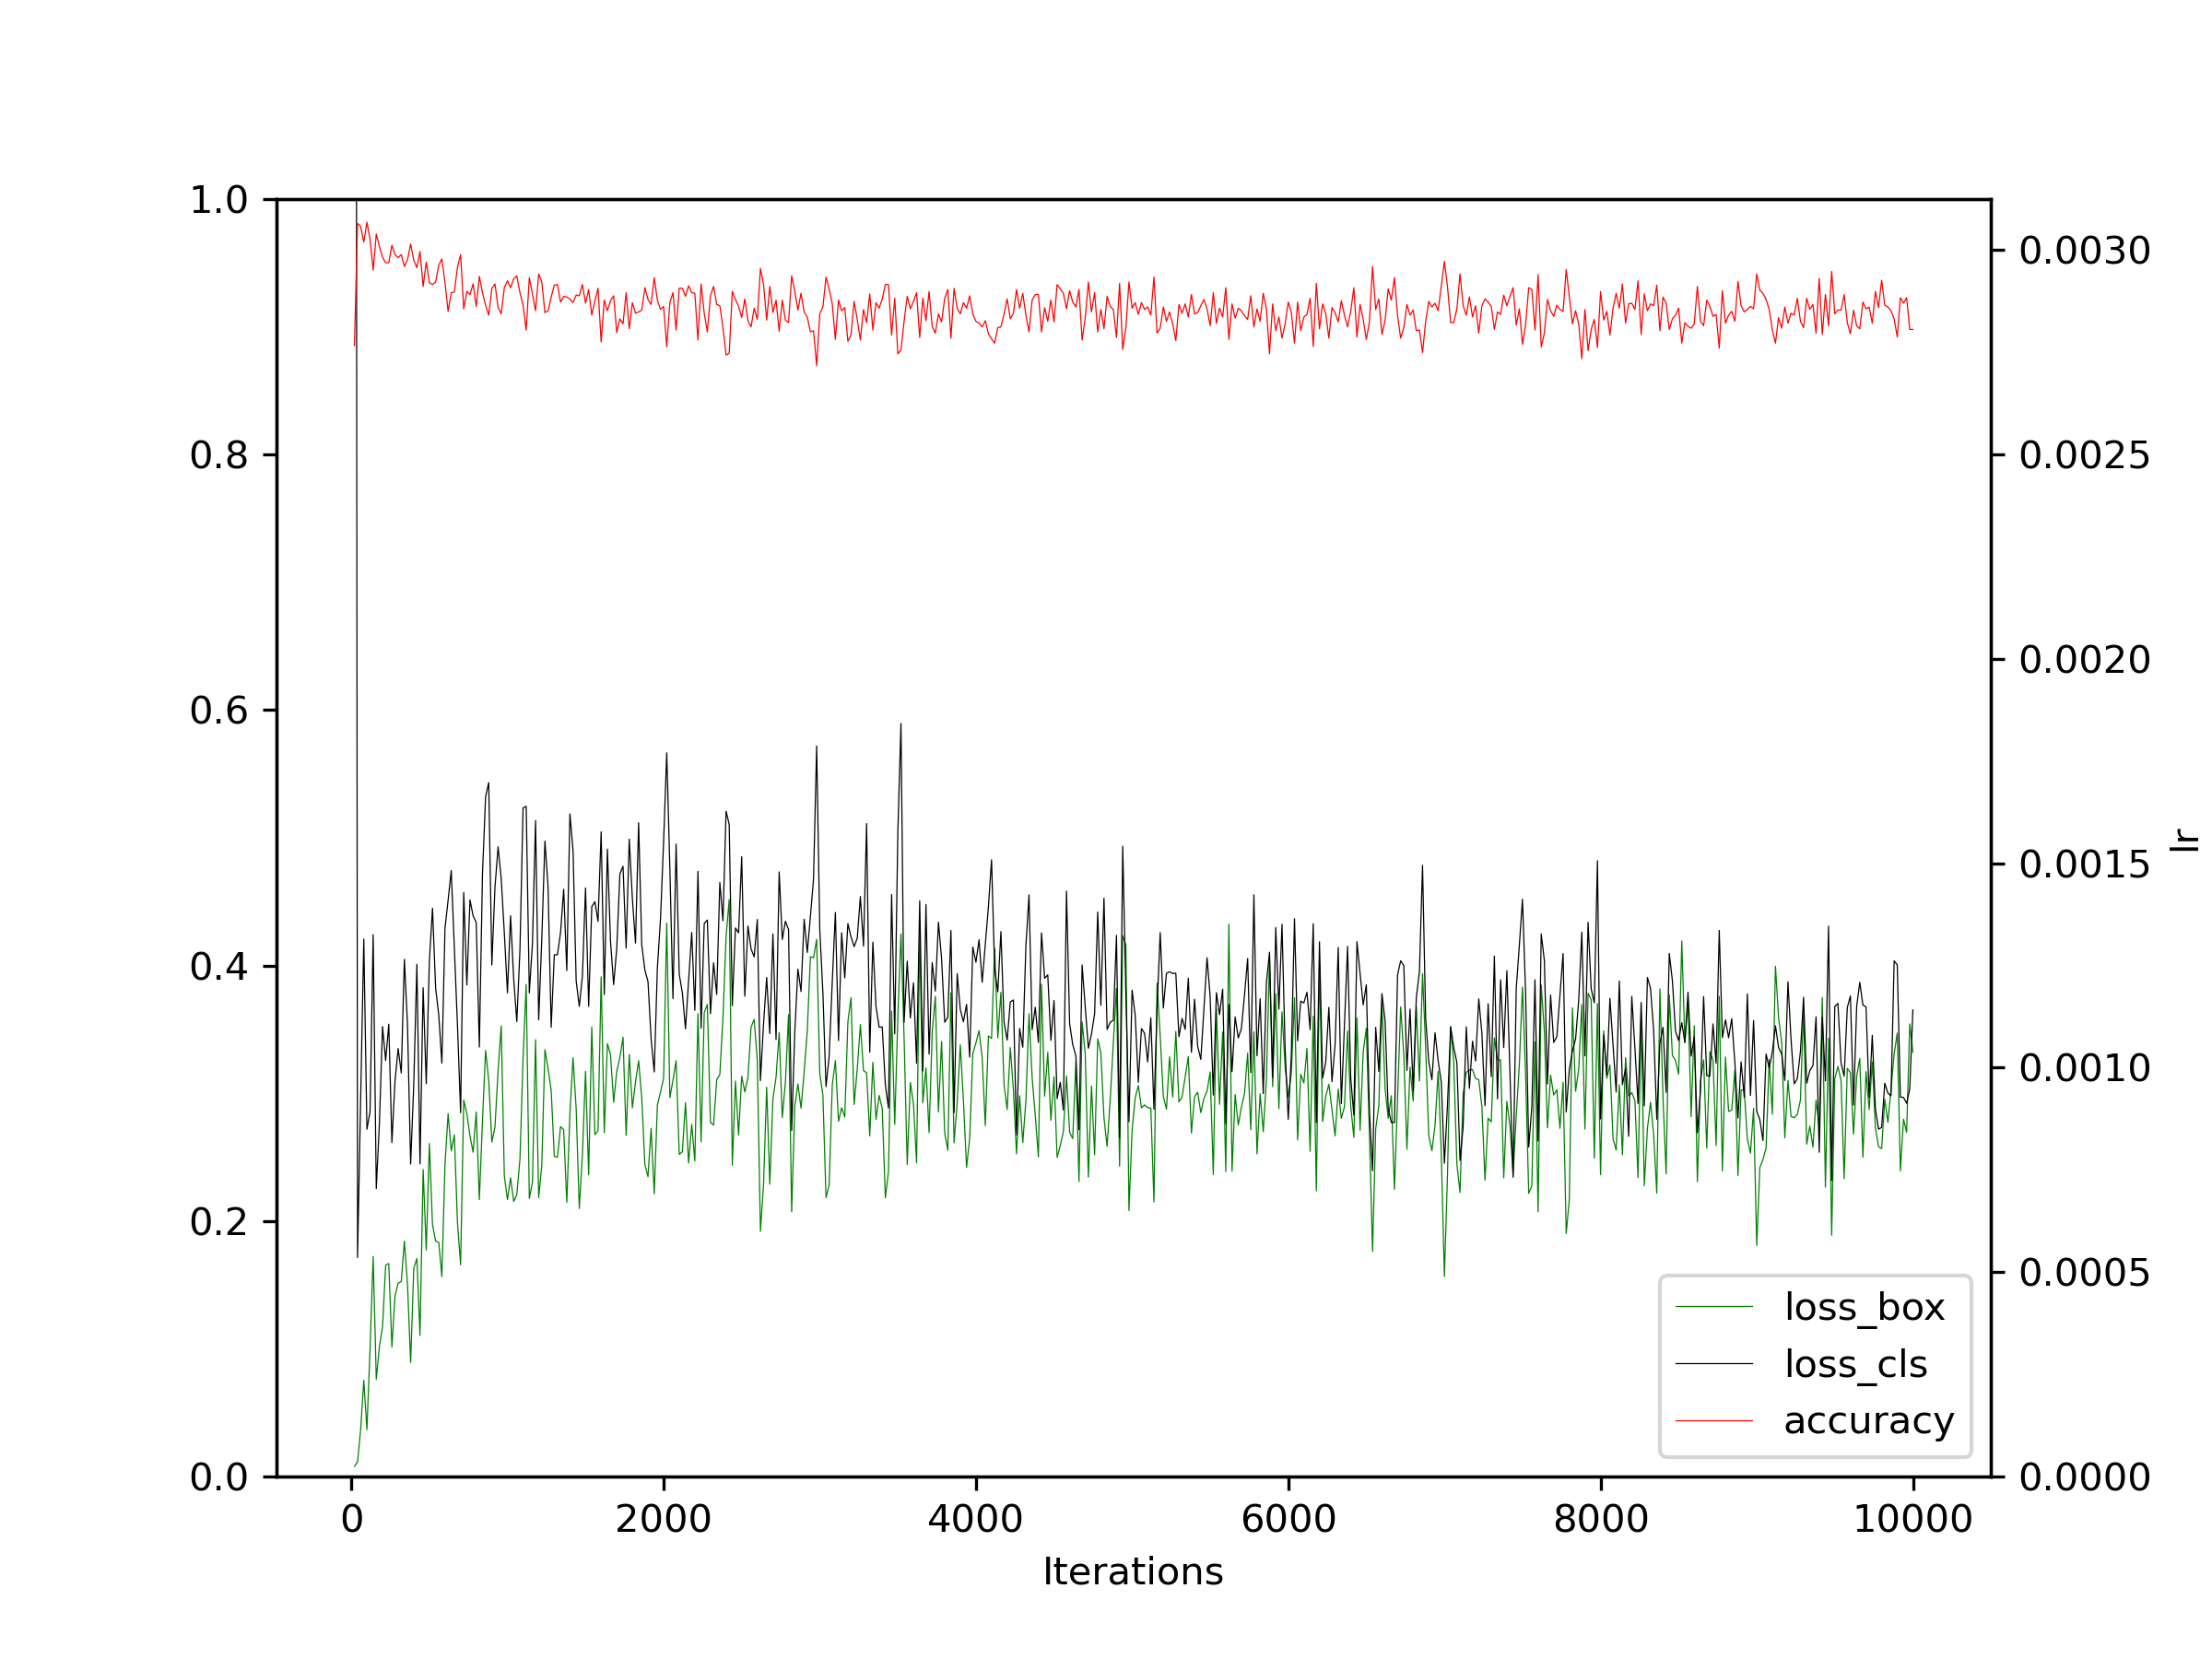
\includegraphics[width=1\textwidth]{figures/faster_rcnn_r_50_fapn_1x_10000iter.png}
    \caption{Faster RCNN \& FaPN with 10000 interactions}\label{faster_rcnn_r_50_fapn_1x_10000iter}
\end{figure}

%可以看出,无论是使用Mask RCNN还是Faster RCNN加上FaPN在COCO2017数据集上进行训练,在10000 iterations下都能得到较高的准确率和较好的性能,具有较强的实用性。
It can be seen that whether Mask RCNN \cite{he2017mask} or Faster RCNN plus FaPN is used for training on the COCO2017 dataset, higher accuracy and better performance can be obtained under 10,000 iterations, and it has strong practicability.

%但COCO2017数据集对于道路交通标识的本地化并不十分有好,其对于国内路标的预测结果很差。

\begin{table}[htb]
% h-here,t-top,b-bottom,优先级依次下降
    \begin{center}
    % 居中
        \caption{Performance of the Faster RCNN on category pedestrian}\label{table1}
        \begin{tabular}{|c|c|c|c|c|c|c|} % 三线表不能有竖线,l-left,c-center,r-right
            \toprule
            %三线表-top 线
            \textbf{Method} & \textbf{Backbone}&\textbf{Iterations} & $AP$ & $AP_s$ & $AP_m$ & $AP_l$ \\
            \hline
            %三线表-middle 线
            FaPN          & \multirow{5}{*}{Faster R-CNN R50}&10K &10.1&5.3&11.4&11.9 \\
            FaPN          &  &20K&12.6&9.5&12.8&15.7 \\
			FaPN (fully trained)         & &65K &40.2&23.9&43.9&48.8 \\
			FaPN (authors')         &  &-&39.2&24.5&43.3&49.1 \\
			FPN  & &- &37.9&22.4&41.1&49.1 \\
            \bottomrule
            %三线表-底线
        \end{tabular}
    \end{center}
\end{table}

\begin{table}[htb]
	% h-here,t-top,b-bottom,优先级依次下降
		\begin{center}
		% 居中
			\caption{Performance of the Mask RCNN on category pedestrian}\label{table2}
			\begin{tabular}{|c|c|c|c|c|c} % 三线表不能有竖线,l-left,c-center,r-right
				\toprule
				%三线表-top 线
				\textbf{Method} & \textbf{Backbone}&\textbf{Iterations} & $AP^{mask}$ & $AP^{mask}_s$ \\
				\hline
				%三线表-middle 线
				FaPN & \multirow{5}{*}{Mask R-CNN R50}&10K&9.5&4.0 \\
				FaPN & &20K&14.4&5.9 \\
				FaPN (fully trained) & &80K &37.2&18.3 \\
				FaPN (authors') & &- &36.4&18.1 \\
				FPN & &- &35.2&17.1 \\
				\bottomrule
				%三线表-底线
			\end{tabular}
		\end{center}
	\end{table}


\subsubsection{Paddle Lite}
Paddle Lite \cite{paddlelite} is an end-to-end reasoning engine launched by Paddle Mobile based on the new upgrade of Paddle Mobile. It is more complete in the support of multi-hardware, multi-platform, and hardware hybrid scheduling, and provides efficient and lightweight AI applications for end-side scenarios including mobile phones. Reasoning ability, effectively solve problems such as mobile phone computing power and memory limitations are committed to promoting the wider implementation of AI applications.

\subsubsection{Model Deployment}
%对于训练好的模型,我们可以得到它的检查点(pth)文件,这个文件保存了模型的所有参数。如果我们需要对一个已经训练的模型进行deploy或者评估,只需要用到对应模型的pth文件即可。

For a trained model, we can get its checkpoint (.pth) file, which holds all the parameters of the model. If we need to deploy or evaluate a trained model, we only need to use the checkpoint file of the corresponding model.
%对于服务器端,我们需要一个通信模块。该模块的功能是接收前端的数据并完成处理,调用相应模型完成对于图片的语义分割,最后将分割好的图片返回给客户端。

For the server-side, we need a communication module. The function of this module is to receive the front-end data and complete the processing, call the corresponding model to complete the semantic segmentation of the image, and finally return the segmented image to the client.

%本服务器端采用的是socket server框架,其基本思想是监听服务器的指定端口。在接收到客户端的连接请求后与其进行握手,建立连接。然后接收并处理相关信息,调用模型。

The server-side adopts the socket server framework, and its basic idea is to monitor the specified port of the server. After receiving the connection request from the client, it makes a handshake with it to establish a connection. Then receive and process the relevant information and call the model.

% \begin{algorithm}[htb]
%     \caption{Pseudo-Code of Model Running Script}
%     \label{alg:Framwork}
%     \begin{algorithmic}[1]
%       \Require
%         The model to run, $M$;
%         The Message-Digest5 check code of the corresponding file, $M_i$;
%         Image file for semantic segmentation, decoded as bitstream is enquired, $F_i$;
%         Either running on \textit{CPU} or GPU, $T$;
%       \Ensure
%         The processed image, $F^p_i$;

%     \end{algorithmic}
% \end{algorithm}


\begin{algorithm} 
	\caption{Pseudo-Code of Model Running Script} 
	\label{alg3} 
	\begin{algorithmic}
		\REQUIRE 
        The model to run, $M$;\ The Message-Digest 5 check code of the corresponding file, $M_i$;
        \ Image file for semantic segmentation, decoded as bitstream is required, $F_i$;
		\ENSURE 
        The processed image, $F^p_i$;
		\STATE Perform the connection procedure with the mobile terminal and hold the connection $Conn$.
		\IF{$M_i$ not equals to any of the existing file $M_e$}
        \STATE $Size_f \gets received\  file\  size$
        \STATE $Recv_f \gets 0$ 
        % \WHILE{$N \neq 0$} 
        % \ENDWHILE
		\ELSE 
		\STATE Return the existing result image.
		\ENDIF
		\WHILE{$Recv_f \neq Size_f$}
		\STATE Hold the connection and continuously receive the file.
		\ENDWHILE 
		\STATE Check the type of the module $M$.
		\STATE Run the module $M$.
		\STATE Return the result image, $F^p_i$.

	\end{algorithmic} 
\end{algorithm}



\subsection{Client End Construction}
%考虑到Android平台庞大的用户群体,广阔的市场和安卓开发的开放性,设计基于Android系统的APP更具有实用性。并且安卓开发人员的基数较大,有利于对APP的针对性优化和系统的完善。基于上述原因,本APP将使用Android作为平台进行实现和完善。
Considering the huge user group of the Android platform, the broad market, and the openness of Android development, it is more practical to design an APP based on the Android system. And the base of Android developers is relatively large, which is conducive to the targeted optimization of the APP and the improvement of the system. For the above reasons, this APP will be implemented and improved using Android as the platform.

%进行基于Android的语义分割APP的开发,主要需要的内容有:1)针对用户需求进行分析,并根据结果设计系统的完整架构。2)和服务器端的接口进行对接,在TCP的基础上实现与服务器端的稳定连接。3)实现所需要的系统功能,包括图像采集处理模块,移动端模型调用模块,数据处理和传输模块,客户端服务器端通信模块等。

To develop an Android-based semantic segmentation APP, the main contents are:
1) Analyze user needs and design the complete architecture of the system according to the results.
2) Connect with the interface of the server, and realize a stable connection with the server based on TCP. 
3) Realize the required system functions, including image acquisition and the processing module, mobile model calling module, data processing, and transmission module, client-server communication module, etc.

\subsubsection{System Structure}
%客户端采用基于Android平台开发,使用原生Java语言进行开发。Android开发主要有两种架构模式:MVC和MVP。为了系统的易于维护性和可扩展性,本APP采用更流行的MVP架构进行开发。相对于传统的MVC框架,主要代码逻辑和工作都堆积在Controller层进行,MVP框架合理分配了View,Presenter和Model三层的压力,实现了代码的解耦。项目的主要逻辑是用户通过点击按钮或者选择选项为View层提供用户输入,View层通过presenter层的接口来更新,Presenter访问Model层来更新或修改数据。这样避免了传统的MVC框架中Activity层中需要同时绑定Activity和View中的事务处理事件和按钮等对象的绑定造成的代码臃肿,同时还通过View层的组件化提高了View层的复用性。

%mvp图形解释

\begin{figure}[htb]
    \centering
    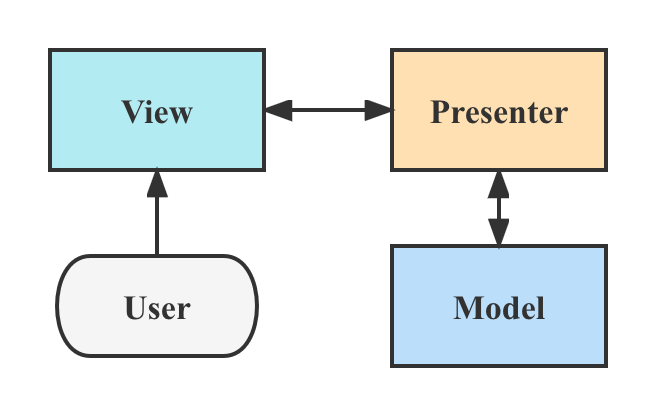
\includegraphics[width=0.5\textwidth]{figures/MVP.png}
    \caption{Illustration of \textit{MVP} framework
 }\label{MVP}
\end{figure}

The client is developed based on the Android platform and is developed using the native Java language. There are two main architectural patterns for Android development: \textit{MVC} and \textit{MVP} \cite{lou2016comparison}. For the ease of maintenance and scalability of the system, this APP adopts the more popular \textit{MVP} architecture for development. Compared with the traditional \textit{MVC} framework, the main code logic and work are accumulated in the Controller layer. The \textit{MVP} framework reasonably allocates the pressure of the View, Presenter, and Model layers to realize the decoupling of the code. The main logic of the project is that the user provides user input to the View layer by clicking buttons or selecting options, the View layer is updated through the interface of the presenter layer, and the Presenter accesses the Model layer to update or modify data. This avoids the bloated code caused by the need to bind transaction processing events and buttons in the Activity layer in the traditional \textit{MVC} framework at the same time and also improves the reuse of the View layer through the componentization of the View layer reusability.


\subsubsection{UI Design}
%前端APP的UI界面需要为用户提供方便易用的主界面和清晰的dense prediction的结果的展示。考虑到本文所指的APP的主要目的是展示语义分割的结果,所以未提供用户登陆界面。

The UI interface of the front-end APP needs to provide users with an easy-to-use main interface and a clear display of the results of dense prediction. Considering that the main purpose of the APP referred to in this article is to display the results of semantic segmentation, the user login interface is not provided.


%语义分割APP的搭建主要分为几部分。其中包括前端APP的UI界面的搭建,该界面需要为为用户提供方便易用的主界面和清晰的dense prediction的结果的展示。语义分割APP还提供了设置页面,针对用户的需求不同可以选择不同的设置。

The construction of the semantic segmentation APP is mainly divided into several parts. This includes the construction of the UI interface of the front-end APP, which needs to provide users with an easy-to-use main interface and a clear display of the results of dense prediction. The Semantic Segmentation APP also provides a setting page, and different settings can be selected according to the different needs of users.

%其中主页面的信息主要包括几项:完成语义分割的结果图像,上方的信息主要是模型的相关信息,包括模型名称,CPU线程数,CPU的 power mode(如果使用了CPU进行语义分割)下方的信息会在处理成功后显示,主要显示了总共处理的时间(以毫秒为单位)

The information on the main page mainly includes several items: the resulting image of the semantic segmentation. The information above is mainly the relevant information of the model, including the model name, the number of \textit{CPU} threads, and the power mode of the \textit{CPU} (if the \textit{CPU} is used for semantic segmentation). Information will be displayed after successful processing, mainly showing the total processing time (in milliseconds).

%选项设置中主要包括了模型的选择选项,CPU的设置选项和输入图像的通道选项。

The option settings mainly include model selection options, \textit{CPU} setting options, and input image channel options.

%对于模型的选择选项,可供选择的选项有选择一项预先训练好的模型,选择是否开启 custom setting,选择内置模型,label,image的path(因为目前只有一个移动端模型,所以这些选项均为提前设置好的)

For the model selection option, the available options include choosing a pre-trained model, choosing whether to enable the custom setting, and choosing the built-in model, label, and image path (because there is currently only one mobile model, these options are all pre-set)

%对于CPU的设置选项,CPU可供选择的线程数包括1,2,4,8,一共四种。CPU power mode有high,low,full三种可供用户选择,它们分别使用手机的大核,小核和all available cores。

For the setting options of the \textit{CPU}, the number of threads available for the \textit{CPU} includes 1, 2, 4, and 8, a total of four. There are three \textit{CPU} power modes: high, low, and full for users to choose from, which use the large core, small core, and all available cores of the mobile phone respectively.

%对于输入图像的通道选项这一项,COCO格式数据集默认图像的通道顺序均为RGB,考虑到用户上传的图片中可能存在BGR通道顺序的图像,因此提供了上传BGR通道图像的选项。

For the channel option of the input image, the default image channel order of the COCO format dataset is RGB. Considering that there may be images in the \textit{BGR} channel order in the images uploaded by the user, the option to upload the \textit{BGR} channel image is provided.

%值得一提的是,因为移动端预训练模型只有paddle lite,且预训练模型的信息均为已知。所以以上选项均已预先设置好,无法进行更改,选项提供关于模型路径的设置选项是考虑到APP的扩展性和可移植性。

It is worth mentioning that because the mobile pre-trained model is paddle lite only, and the relevant information of the pre-trained model is known. Therefore, the above options are pre-set and cannot be changed. The option to provide setting options for the model path is to take into account the scalability and portability of the APP.

\subsection{Main Module Calling Logic}
%APP主要模块有几个:模型调用模块,图像采集和处理模块,数据传输模块,分别承担了加载和启动模型并将获取到的数据送入模型中;从相册或相机API获取图像并送入所需要的下一个模块中;将获取到的图像分发给服务器端并监听服务器端的回传数据。

There are several main modules of the APP, model calling module, image acquisition, and processing module, and data transmission module, respectively responsible for loading and starting the model and sending the obtained data into the model; obtaining images from the album or camera API and sending them to the required next module, distribute the obtained image to the server-side and monitor the return data from the server-side.

%对于可能的优化方向,可以考虑调用相机后,获取实时的视频,将从视频中截取的特定帧直接送到分割模型,图片完成分割后自动退出相机将分割图展示到界面进行上传,采用这种方式,会让整个系统更加简单与智能,同时也可以减少用户所需要的操作步骤,使得整个图片分割的时间缩短,提升用户的使用体验。

As for possible optimization directions, consider calling the camera to obtain a real-time video, and directly send the specific frame captured from the video to the segmentation model. After the image is segmented, automatically exit the camera and display the segmentation image on the interface for uploading. This method would make the whole system simpler and smarter, and at the same time, it can reduce the operation steps required by the user, shorten the time for the entire image segmentation, and improve the user experience.

\subsubsection{Model Invocation Module}
%模型调用模块调用的是APP内置的Paddle Lite模型,通过createPaddlePredictor来加载预先训练好的模型。每次加载模型前要先release之前的模型,以避免模型的相关设置(thread num等)与先前的模型设置产生冲突。然后通过加载设置中的Power Mode和Thread Num的相关信息对模型进行初始化,在模型初始化完成后就可以对模型进行调用和其他任务的执行。

The model calling module calls the built-in Paddle Lite model of the APP and loads the pre-trained model through \textit{createPaddlePredictor}. Before each model is loaded, the previous model must be released to avoid conflicts between the related settings of the model (thread num, etc.) and the previous model settings. Then initialize the model by loading the relevant information of Power Mode and Thread Num in the settings. After the initialization of the model is completed, the model can be called and other tasks can be executed.


\begin{algorithm} 
	\caption{Pseudo-Code of Model Calling Algorithm} 
	\label{alg4} 
	\begin{algorithmic}
		\REQUIRE 
        The model to run, $M$;\ 
		Settings of the model, $S = [s_1, s_2, ..., s_n]$
		\ENSURE 
        The processed image, $F^p_i$;
		\STATE Start a new thread.
		\STATE Check if the model to run is the transplanted model or the server-side model.
		\IF{$M$ is the transplanted model}
        \STATE Initialize the model.
		\STATE Pass the $S = [s_1, s_2, ..., s_n]$ to the model and start the timer.
		\STATE Use the handle to keep listening until the returned image is received.
		\STATE $F^p_i \gets the\  received\  image$
		\STATE End the timer and calculate the total processed time.
		\ELSE 
		\STATE Calculate and transfer the MD5 of the given image.
		\IF{the file has been processed before}
		\STATE $F^p_i \gets the\  received\  image$
		\ENDIF
		\ELSE
		\STATE Transfer the image.
		\WHILE{not all data has been received}
		\STATE Hold the connection and continuously receive the file.
		\ENDWHILE 
		\ENDIF
		\STATE Return the result image, $F^p_i$.

	\end{algorithmic} 
\end{algorithm}

\subsubsection{Image Acquisition and Processing Module}
%图像采集和处理模块的主要功能是收集要用于语义分割的图像,并将其送入数据传输或者模型调用模块进行处理。安卓端主要有两种获取图像的方式:通过相册获取本地图库中的照片,通过调用手机摄像头API实时拍摄照片。两种方式的入口均在右上角的更多选项中。在用户点击Open Gallery或者Take Photo之后,重写的onOptionsItemSelected方法会通过安卓自带的Manifest获取相册或者摄像头的权限,然后根据相应选择打开相册或者摄像头。在第一次使用时手机会弹出相应弹框供用户进行确认,在用户确认后即可使用相关权限。

\begin{figure}[htb]
    \centering
    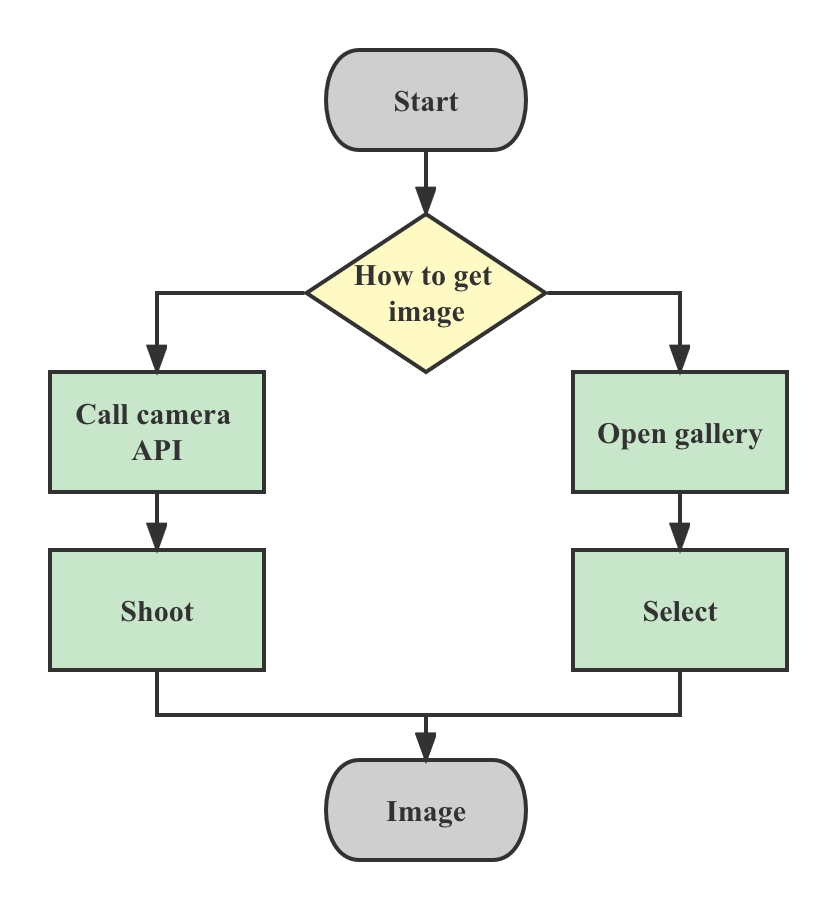
\includegraphics[width=0.5\textwidth]{figures/pictureget.png}
    \caption{Flowchart of picture acquisition module}\label{pictureget}
\end{figure}

The main function of the image acquisition and processing module is to collect the images to be used for semantic segmentation and send them to the data transmission or model calling module for processing. There are two main ways to obtain images on the Android side: obtain photos in the local gallery through the photo album, and take photos in real-time by calling the mobile phone camera API. The entrance to both ways is in the more options in the upper right corner. After the user clicks Open Gallery or Take Photo, the rewritten \textit{onOptionsItemSelected} method will obtain the permission of the album or camera through the Manifest that comes with Android, and then open the album or camera according to the corresponding selection. When using it for the first time, the mobile phone will pop up a corresponding pop-up box for the user to confirm, and the relevant permissions can be used after the user confirms.

%如果选择的是Take Photo,那么通过调用系统自带的Intent Action ACTION_IMAGE_CAPTURE可以获取到相机APP的Intent,开启startActivityForResult后,用户就可以通过相机拍摄自己所需要的照片。这时APP通过onActivityResult对拍摄过程进行监听,当用户的拍摄行为结束后,onActivityResult可以获取到用户行为的相关信息,然后通过判断用户是否正常进行了拍照流程来判断是否将获取到的图像传给模型调用模块。

If Take Photo is selected, the Intent of the camera APP can be obtained by calling the Intent Action \textit{ACTION\_IMAGE\_CAPTURE} that comes with the system. After startActivityForResult is enabled, the user can take the photos they need through the camera. At this time, the APP monitors the shooting process through \textit{onActivityResult}. When the user's shooting behavior ends, \textit{onActivityResult} can obtain the relevant information of the user's behavior, and then judge whether the obtained image is passed to the model by judging whether the user has performed the shooting process normally. Call the module.

%如果选择的是Open Gallery,那么通过系统自带的ACTION_PICK的Intent Action来选择手机特定资源路径下的文件,我们知道手机相册的type是image/*,那么通过setDataAndType就可以获取外部资源库的相册的资源,然后再通过onActivityResult对用户选择图像的行为进行监听,当监听器获取到返回值后,就可以根据相应的反回信息进行判断,并进行下一步的模型加载和图像分割工作。

If you choose Open Gallery, then use the Intent Action of \textit{ACTION\_PICK} that comes with the system to select the file under the specific resource path of the mobile phone. We know that the type of the mobile phone album is \textit{image/*}, then you can get the album of the external resource library through \textit{setDataAndType}, resources, and then monitor the user's behavior of selecting images through \textit{onActivityResult}. When the listener obtains the return value, it can judge according to the corresponding return information, and carry out the next model loading and image segmentation work.

\subsubsection{Data Transmitting Module}
%数据传输模块的主要功能是向服务器端发送执行运行模型命令和发送需要处理的图像。接收并编码处理完成的图像并对其进行相应处理并传给UI模块以供显示。

The main function of the data transmission module is to send the execution model command to the server and send the image to be processed \cite{rhodes2014foundations}. The processed image is received and encoded and processed accordingly and passed to the UI module for display.

%在接收到图像处理模块发来的相关信息后,数据传输模块会先启动一个子线程。子线程启动后与指定IP和端口的服务器端进行连接,并hold连接等待传输。在握手完成后首先传输图像的md5值供服务器进行判断,在服务器端返回确认可以不存在图像的命令后,传输等待处理的图像,然后等待接收processed图像。将接收到的字节流encode之后将结果传输至UI模块以供结果的显示。


After receiving the relevant information from the image processing module, the data transmission module will first start a sub-thread. After the child thread starts, it connects to the server with the specified IP and port and holds the connection to wait for transmission. After the handshake is completed, the md5 value of the image is first transmitted for the server to judge. After the server returns a command to confirm that there is no image, the image waiting to be processed is transmitted, and then the processed image is received. Encoding the received byte stream, the result is transmitted to the UI module for display of the result.


% \subsection{APP Results and Analysis}

% \begin{figure}[htbp]
%     \centering
%     \begin{subfigure}[t]{0.4\linewidth}
%         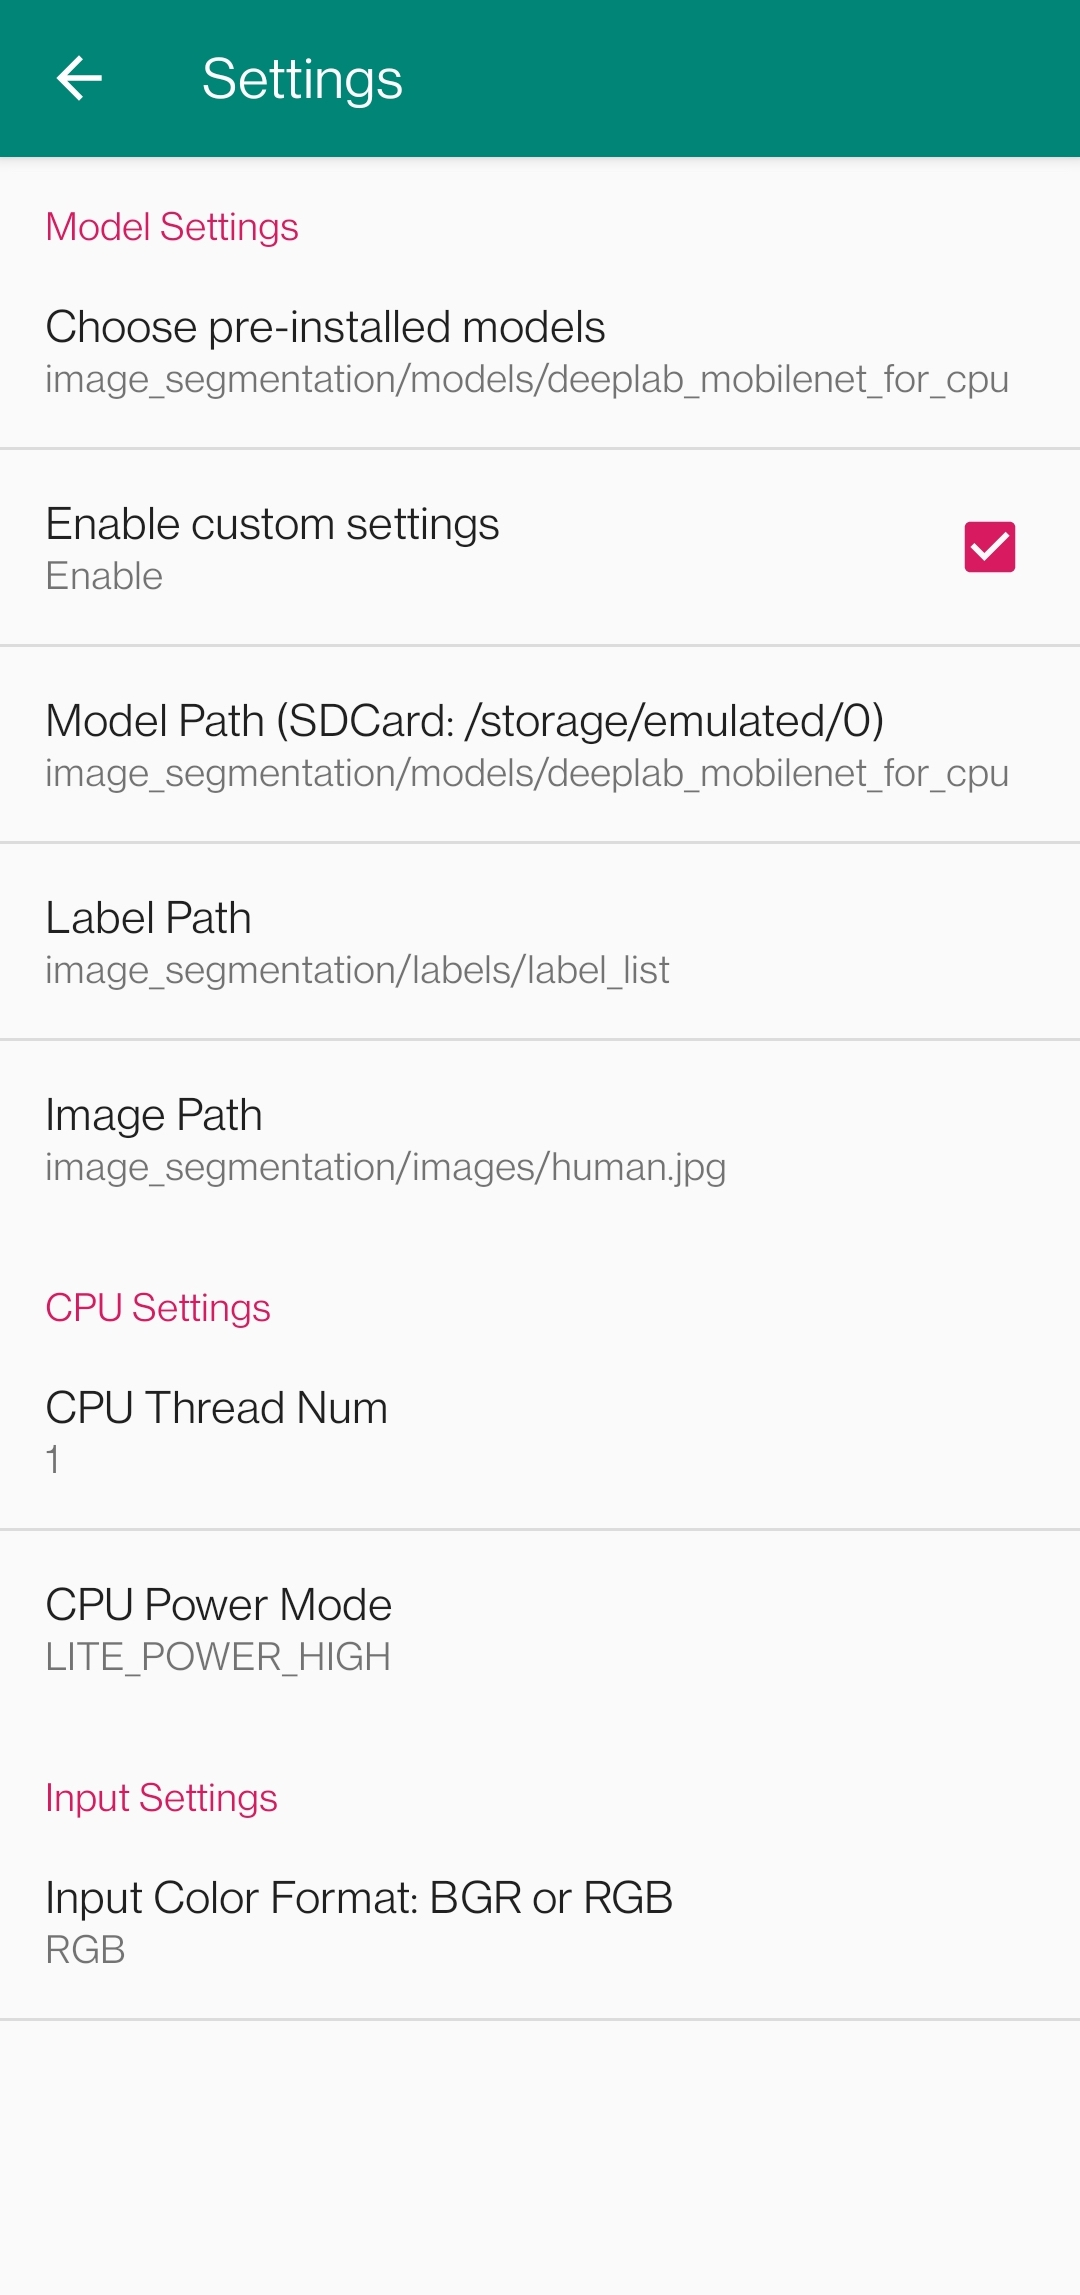
\includegraphics[width=1\textwidth]{figures/settings.jpg}
%         \caption{The Whole Settings Page}\label{settings}
%     \end{subfigure}
%     \begin{subfigure}[t]{0.4\linewidth}
%         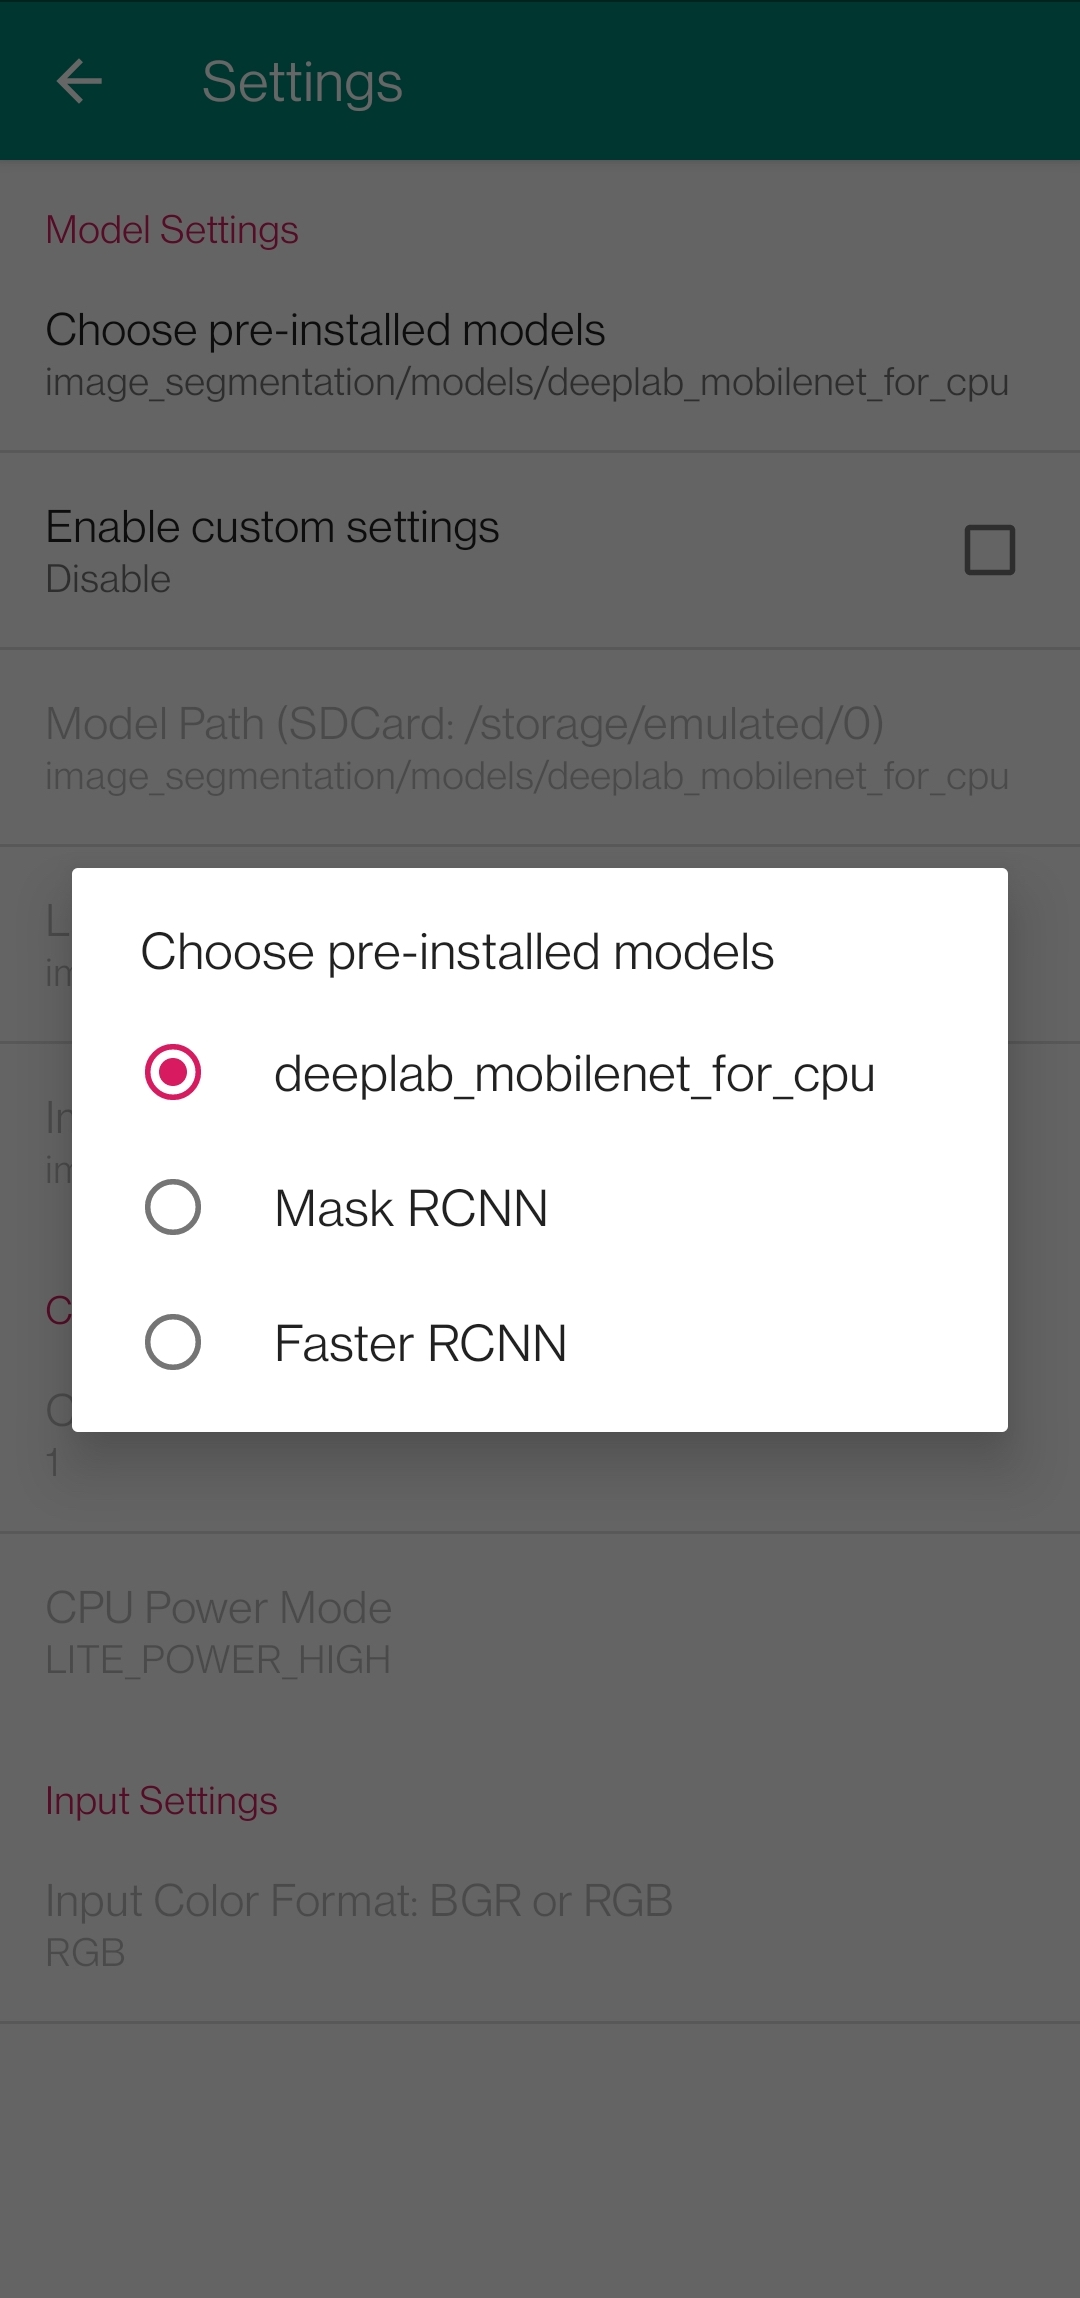
\includegraphics[width=1\textwidth]{figures/type.jpg}
%         \caption{Selection Setting about Pre-installed Models}\label{type}
%     \end{subfigure}
%     \caption{Settings Pages}\label{result1}
% \end{figure}

% \begin{figure}[htbp]
%     \centering
%     \begin{subfigure}[t]{0.3\linewidth}
%         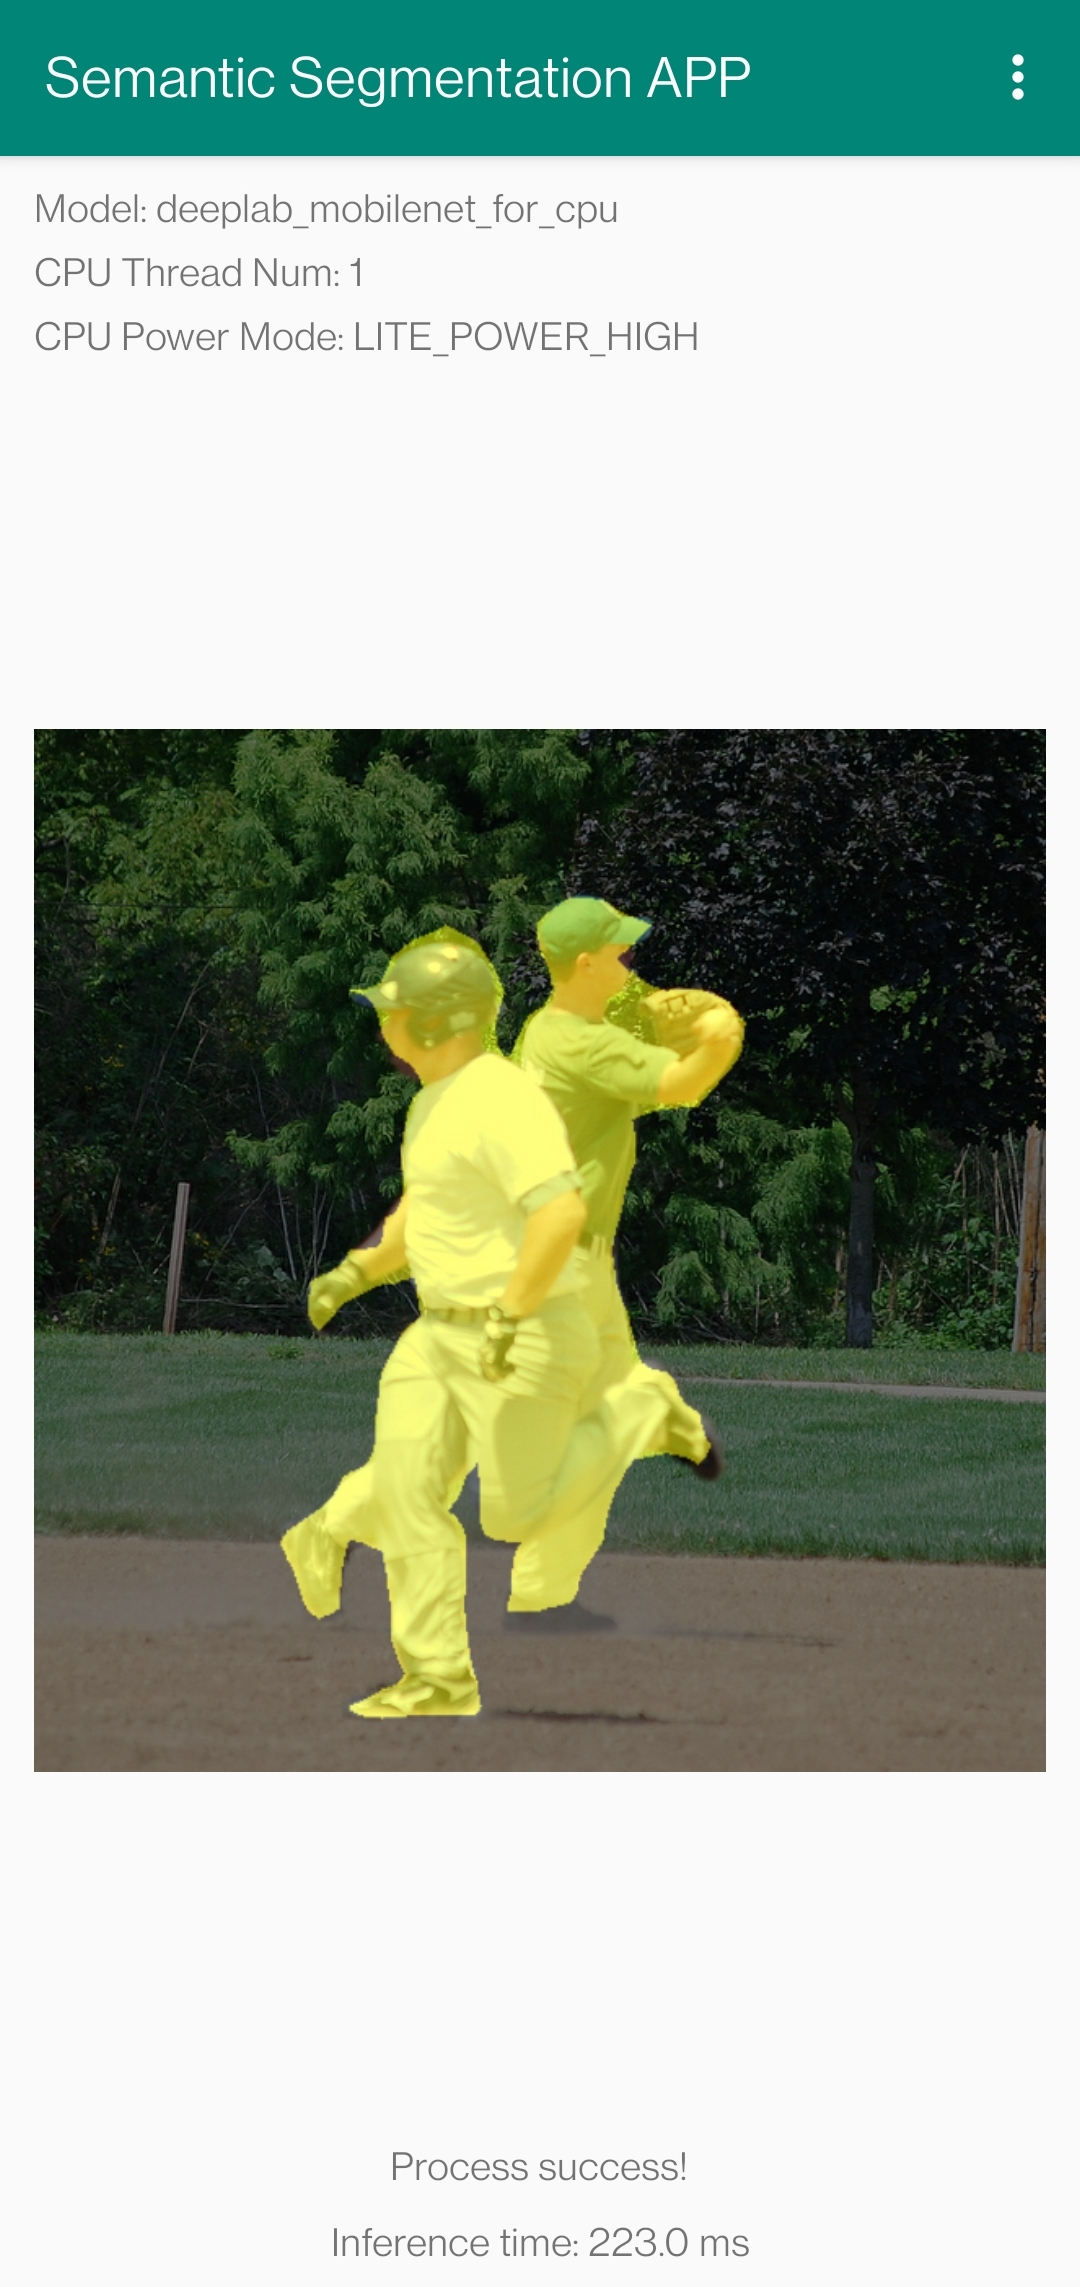
\includegraphics[width=1\textwidth]{figures/paddleresult.jpg}
%         \caption{Segmentation Result of Paddle Lite}\label{resultpaddle}
%     \end{subfigure}
%     \begin{subfigure}[t]{0.3\linewidth}
%         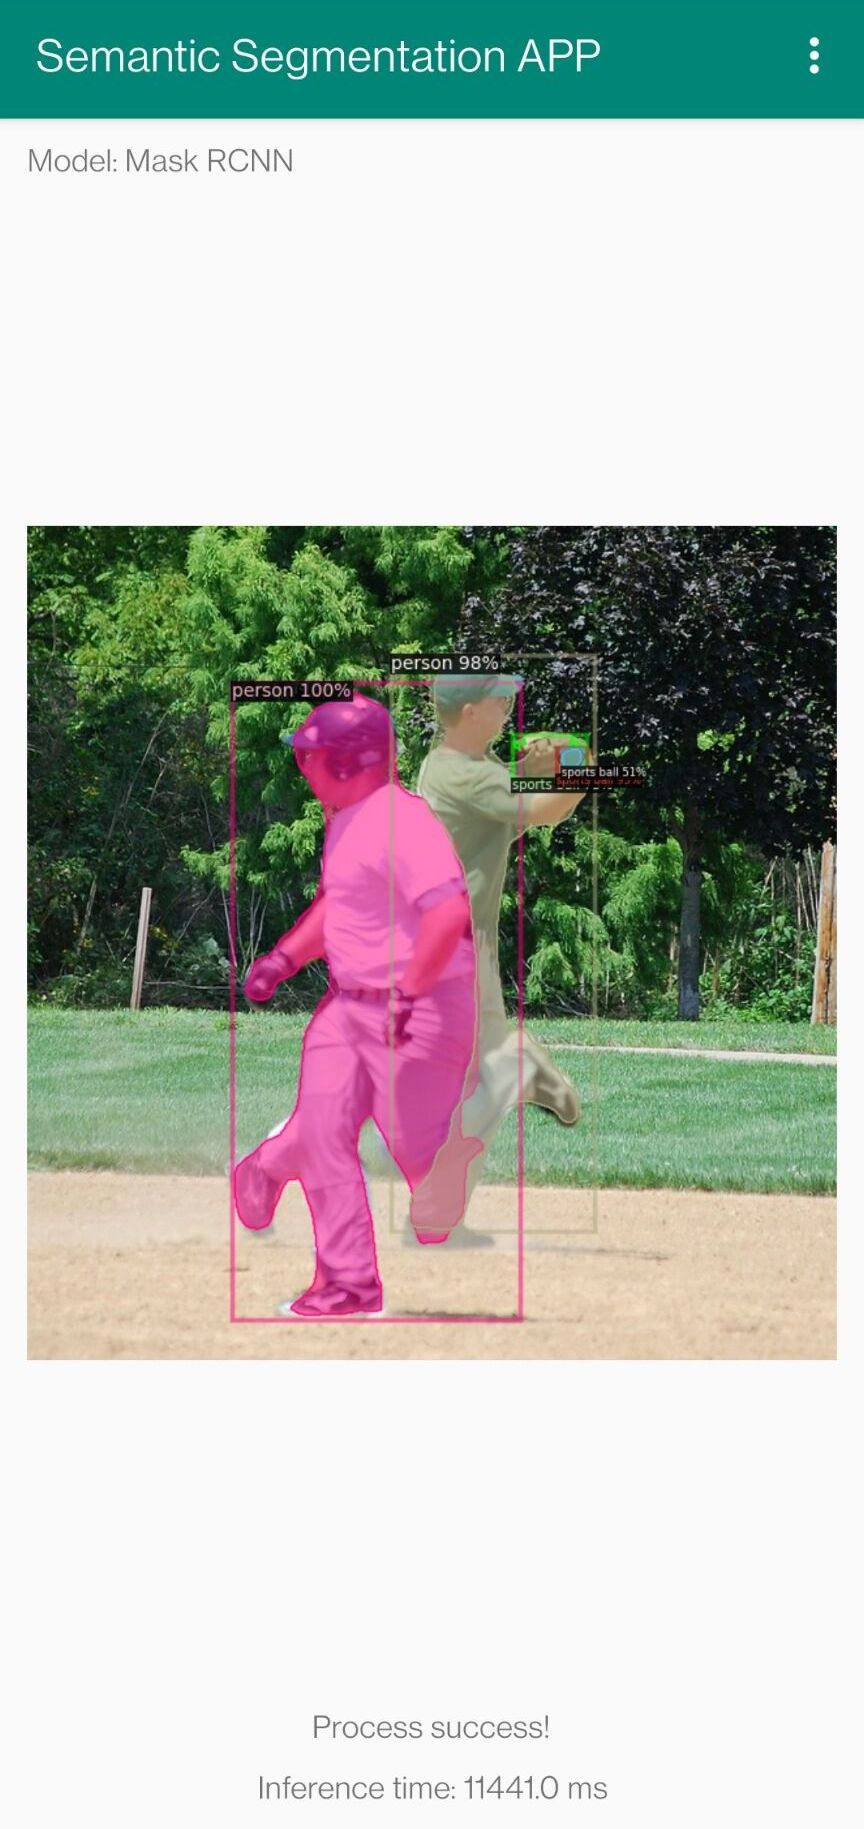
\includegraphics[width=1\textwidth]{figures/maskresult.jpg}
%         \caption{Segmentation Result of Mask RCNN}\label{resultmaskrcnn}
%     \end{subfigure}
%     \begin{subfigure}[t]{0.3\linewidth}
%         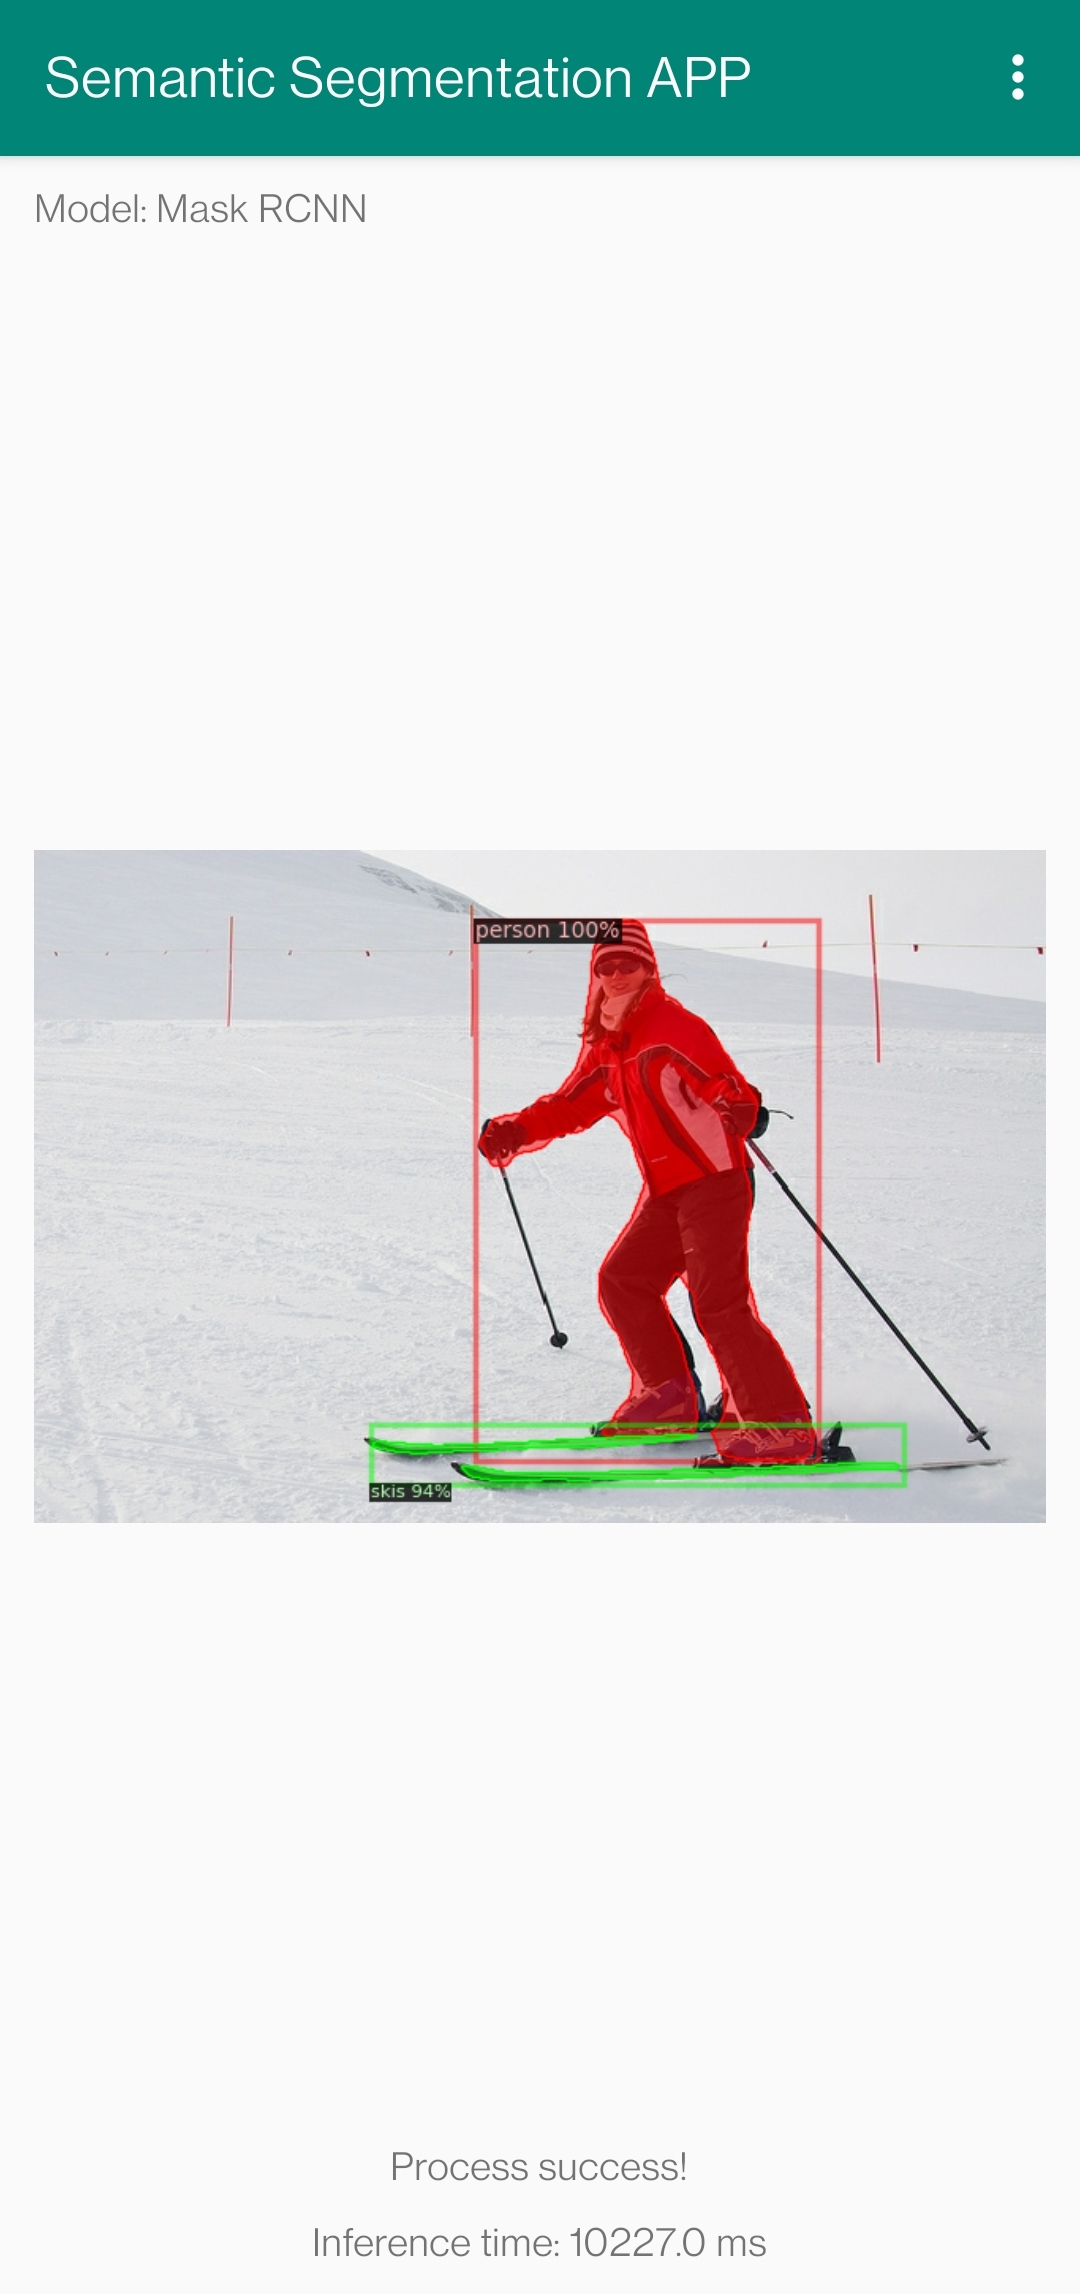
\includegraphics[width=1\textwidth]{figures/ski.jpg}
%         \caption{Segmentation Result of Mask RCNN}\label{resultskimaskrcnn}
%     \end{subfigure}
%     \caption{Result With Different Model and Images}\label{result2}
% \end{figure}

% %该部分选取了APP的设置页面和分割结果予以展示。设置页面提供了对于模型的选项,用户可以在设置页面里选择模型的路径,图像的路径和通道顺序等等。对于结果来说,可以看到对于物体及其边界的识别的效果较好,而对于实力分割中同类的存在重叠物体的边界识别还存在问题。但是对于单独物体的识别和分割的效果较好,达到了预期。

% This part selects the settings page of the APP and the segmentation results to display. The settings page provides options for the model, the user can choose the path of the model, the path of the image and the channel order, etc. in the settings page. For the results, it can be seen that the recognition of objects and their boundaries is better, but there are still problems in the recognition of the boundaries of overlapping objects of the same kind in strength segmentation. However, the effect of recognition and segmentation of individual objects is better, which has reached the expectation.

% %其中可以看到在使用非预移植模型时,处理所需的时间较长。其中对于尺寸较大的图片,80%左右的时间用于数据传输,10%左右的时间用于加载模型,10%左右的时间用于分割。对于尺寸较小的图像也仅有50%的时间是真正用于模型的运行。模型运行的效率约为$2s/Obj$

% It can be seen that the processing time is longer when using the non-preported model. Among them, for large-sized images, about 80\% of the time is used for data transmission, about 10\% of the time is used to load the model, and about 10\% of the time is used for segmentation. For smaller images, only 50\% of the time is actually used for running the model. The model runs with an efficiency of about $2s/Obj$.

% % Reference如是\cite{Nicholas1998Handbook}。

\clearpage